\documentclass[journal]{IEEEtran}
\usepackage[utf8]{inputenc}
\usepackage[portuguese]{babel}
\usepackage{url}
\usepackage{booktabs}
\usepackage{graphicx}
\usepackage{multirow}
\usepackage{amsmath}

\begin{document}

\title{
	Comparação de funções de aprendizado no método Backpropagation \\ 
	\large Texto apresentado à disciplina Redes Neurais Artificias \\ 
	Graduação em Engenharia de Sistemas \\
	Universidade Federal de Minas, 2018 01 \\ 
	Professor Antônio Pádua de Braga
}
\author{Matheus Araujo, 2013066265}
\markboth{Redes Neurais Artificias, Trabalho Final}{Matheus Araujo}

\maketitle

\begin{abstract}
O texto a seguir foi apresentado como trabalho final para a disciplina \emph{Redes Neurais Artificiais}, no primeiro semestre de 2018, graduação em \emph{Engenharia de Sistemas}, na \emph{Universidade Federal de Minas Gerais}. Nele duas funções de aprendizado do método Backpropagation são avaliadas e comparadas: a função padrão e a função SCG, Scaled Conjugate Gradient, ou Gradiente Conjugado em Escala. A eficiência das funções foi comparada através da confusion matrix dos resultados obtidos por redes treinadas em condições equiparadas.
\end{abstract}

\section{Introdução}

Para o presente trabalho, apresentado como trabalho final à disciplina de Redes Neurais Artificias, graduação em Engenharia de Sistemas, foi proposto a escolha de cinco bases de dados a fim de verificar o comportamento de redes neurais multicamadas. As bases escolhidas foram: Iris, Letter Recognition, Wine, Tic Tac Toe e Balance Scale. Foi utilizada a ferramenta RStudio, com a linguagem R, bem como o pacote RSNNS.

Nos experimentos foram camparados os métodos Backpropagation Padrão e SCG, os resultados e comparativos são apresentados a seguir.

\section{Revisão de Literatura}

\subsection{Redes Neurais Artificiais}

Redes Neurais Artificiais são sistemas paralelos distribuídos compostos por unidades de processamento simples que executam cálculos matemáticos. Essas unidades são dispostas em uma ou mais camadas e são interligadas por um grande número de conexões, normalmente unidirecionais. As conexões possuem pesos que armazenam o conhecimento adquirido pelo modelo. RNAs têm como procedimento usual uma etapa de aprendizagem, onde um conjunto de exemplos é apresentado a ela. A rede então aprende e generalização a informação \cite{bib-braga}.

\subsection{Backpropagation}

Backpropagation é um algoritmo utilizado para o treinamento de Redes MLP, Multi-Layer-Perceptron. Esse método utiliza o gradiente descendente para calcular o erro das camadas intermediárias através de uma estimativa do efeito que elas causam na camada de saída. No algoritmo, o erro na saída é calculado e é então retroalimentado para as camadas intermediárias, possibilitando o ajuste dos pesos proporcionalmente aos valores das conexões entre as camadas.

\subsection{Scaled Conjugate Gradient}

O algoritmo SCG, Scaled Conjugate Gradient, é um algoritmo de aprendizado supervisionado com taxa de convergência superlinear. Ele utiliza uma técnica de otimização baseada no Gradiente Conjungado. \cite{bib-moller}

\subsection{Confusion Matrix}

A Confusion Matrix, também conhecida como Error Matrix, é uma tabela que permite a visualização da performance de um algoritmo de classificação. Nas colunas são representadas as classes reais e nas linhas as classes calculadas pela rede. Assim, cada célula da matriz representa o cruzamento entre a quantidade real de casos e a quantidade encontrado dos casos. Por consequência, a diagonal principal  da matriz irá representar a quantidade de acertos da rede.

\section{Metodologia Utilizada}

Para avaliar as duas funções a seguinte metodologia foi utilizada:

\begin{enumerate}
	\item $85\%$ dos dados disponíveis foram utilizados para treinar a rede;
	\item Após o treinamento, os $15\%$ dos dados restantes foram avaliados pela rede neural criada;
	\item A confusion matrix dos resultados avaliados foi calculada;
	\item O índice de acertividade foi calculado segundo a fórmula:
	$$ \text{índice acertividade} = \frac{\text{soma diagonal principal}}{\text{soma toda matriz}} $$
	\item Os passos 1 a 4 foram repetidos 10 vezes para cada método e cada base de dados;
	\item A média do índice de acertividade foi então calculada.
\end{enumerate}

Para executar os redes foi utilizado o método \texttt{mlp} do pacote \texttt{RSNNS}. Nesse método o parâmetro \texttt{size} diz respeito à quantidade de neurônios na rede neural. O parâmetro \texttt{learnFuncParams} define paramêtros para as funções de aprendizado. E o parâmetro \texttt{maxtit} define a quantidade máxima de épocas para a etapa de aprendizagem \cite{bib-rsnns}.

As bases de dados utilizadas estão apresentadas a seguir.

\subsection{Iris}

O primeiro problema estudado foi o \emph{Iris} \cite{bib-iris}.

\begin{itemize}	
	\item \textbf{Número de instâncias}: 150
	\item \textbf{Número de atributos}: 4
	\item \textbf{Número de classes}: 3
\end{itemize}

Essa é uma base de dados muito conhecida no ramo de Redes Neurais Artificias. Ela avalia dimensões físicas de espécimes de três classes de plantas iris: Iris Setosa, Iris Versicolour e Iris Virginica.

\subsection{Letter Recognition}

O segundo problema estudado foi o \emph{Letter Recognition} \cite{bib-letter-recognition}.

\begin{itemize}	
	\item \textbf{Número de instâncias}: 20000
	\item \textbf{Número de atributos}: 16
	\item \textbf{Número de classes}: 26
\end{itemize}

Nesse problema as 26 letras do alfabeto inglês são identifacadas em imagens preto e branco de onde foram extraídos 16 atributos numéricos.

\subsection{Wine}

O terceiro problema estudado foi o \emph{Wine} \cite{bib-wine}.

\begin{itemize}	
	\item \textbf{Número de instâncias}: 178
	\item \textbf{Número de atributos}: 13
	\item \textbf{Número de classes}: 3
\end{itemize}

Nesse problema resultados de analíses químicias são usados para determinar a origem de vinhos.

\subsection{Tic Tac Toe}

O quarto problema estudado foi o \emph{Tic Tac Toe} \cite{bib-tic-tac-toe}.

\begin{itemize}	
	\item \textbf{Número de instâncias}: 958
	\item \textbf{Número de atributos}: 9	
	\item \textbf{Número de classes}: 2
\end{itemize}

Nesse problema, todas as possibilidade de um tabuleiro do \emph{Jogo da Velha} onde $x$ começou são mostradas e classificadas quanto à possibilidade do $x$ vencer ou não.

\subsection{Balance Scale}

O quinto problema estudado foi o \emph{Balance Scale} \cite{bib-balance-scale}.

\begin{itemize}	
	\item \textbf{Número de instâncias}: 625
	\item \textbf{Número de atributos}: 4
	\item \textbf{Número de classes}: 3
\end{itemize}

Nesse problema um modelo físico de uma balança é avaliado. Na balança há dois diferentes pesos em diferentes distâncias do centro. Em cada configuração a balança pode estar pendendo para a esquerda, ou para a direita ou equilibrada. 

\section{Resultados}

A seguir são apresentados os resultados das execuções para as bases de dados avaliados.

\subsection{Iris}

\subsubsection{Backpropagation padrão}

O backpropagation padrão foi executado para a base de dados Iris com os seguintes parâmetros:

\begin{itemize}
	\item \texttt{size}: 5
	\item \texttt{learnFuncParams}: 0.1
	\item \texttt{maxit}: 50
\end{itemize}

A confusion matrix de uma execução é apresentada na Figura \ref{figura-confusion-matrix-iris-backpropagation-padrao}.

\begin{figure}[h!]
  \centering
  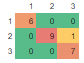
\includegraphics[width=0.3\linewidth]{figs/confusion-matrix-iris-backpropagation-padrao.png}
  \caption{Confusion Matrix - Iris - Backpropagation padrão}
  \label{figura-confusion-matrix-iris-backpropagation-padrao}
\end{figure}

Os resultados para as 10 execuções do backpropagation padrão com as taxas de acertividade são apresentados na Tabela \ref{tabela-resultado-iris-backpropagation-padrao}. A média de acertividade foi de $0.9609$, com desvio padrão de $0.0432$.

\begin{table}[h!]
\centering
\caption{Resultados - Iris - Backpropagation padrão}
\label{tabela-resultado-iris-backpropagation-padrao}
\begin{tabular}{ll}
\toprule
                       & \textbf{Acertividade}       \\ \midrule
Execução 1             & 0.8696          \\
Execução 2             & 0.9130          \\
Execução 3             & 1.0000           \\
Execução 4             & 0.9565          \\
Execução 5             & 1.0000           \\
Execução 6             & 0.9565          \\
Execução 7             & 1.0000           \\
Execução 8             & 1.0000           \\
Execução 9             & 0.9565          \\
Execução 10            & 0.9565          \\ \bottomrule
\textbf{Média}         & \textbf{0.9609} \\
\textbf{Desvio Padrão} & \textbf{0.0432}
\end{tabular}
\end{table}

%O erro iterativo é apresentado na Figura \ref{figura-erro-iterativo-iris-backpropagation-padrao}.

%\begin{figure}
%  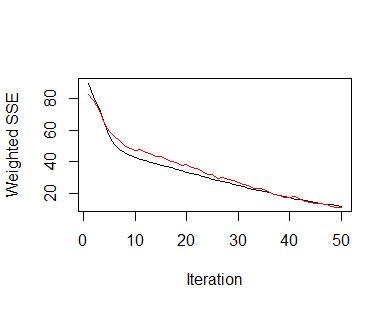
\includegraphics[width=\linewidth]{figs/erro-iterativo-iris-backpropagation-padrao.png}
%  \caption{Erro iterativo - Iris - Backpropagation padrão}
%  \label{figura-erro-iterativo-iris-backpropagation-padrao}
%\end{figure}

\subsubsection{SCG}

O backpropagation com função de aprendizado SCG foi executado para a base de dados Iris com os seguintes parâmetros:

\begin{itemize}
	\item \texttt{size}: 5
	\item \texttt{learnFuncParams}: (0, 0, 0, 0)
	\item \texttt{maxit}: 50
\end{itemize}

A confusion matrix de uma execução é apresentada na Figura \ref{figura-confusion-matrix-iris-backpropagation-scg}.

\begin{figure}[h!]
  \centering
  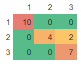
\includegraphics[width=0.3\linewidth]{figs/confusion-matrix-iris-backpropagation-scg.png}
  \caption{Confusion Matrix - Iris - Backpropagation SCG}
  \label{figura-confusion-matrix-iris-backpropagation-scg}
\end{figure}

Os resultados para as 10 execuções do backpropagation SCG com as taxas de acertividade são apresentados na Tabela \ref{tabela-resultado-iris-backpropagation-scg}. A média de acertividade foi de $0.9739$, com desvio padrão de $0.0367$.

\begin{table}[h!]
\centering
\caption{Resultados - Iris - Backpropagation SCG}
\label{tabela-resultado-iris-backpropagation-scg}
\begin{tabular}{ll}
\toprule
                       & \textbf{Acertividade}       \\ \midrule
Execução 1             & 1.0000          \\
Execução 2             & 1.0000          \\
Execução 3             & 0.9565           \\
Execução 4             & 0.9565          \\
Execução 5             & 1.0000           \\
Execução 6             & 1.0000          \\
Execução 7             & 0.9130           \\
Execução 8             & 1.0000           \\
Execução 9             & 1.0000          \\
Execução 10            & 0.9130          \\ \bottomrule
\textbf{Média}         & \textbf{0.9739} \\
\textbf{Desvio Padrão} & \textbf{0.0367}
\end{tabular}
\end{table}

%O erro iterativo é apresentado na Figura \ref{figura-erro-iterativo-iris-backpropagation-scg}.
%
%\begin{figure}
%  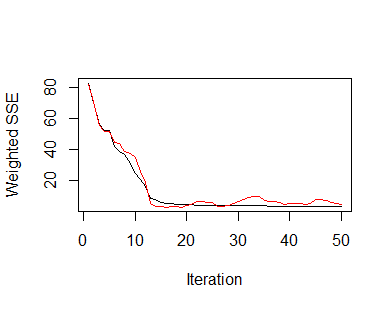
\includegraphics[width=\linewidth]{figs/erro-iterativo-iris-backpropagation-scg.png}
%  \caption{Erro iterativo - Iris - Backpropagation SCG}
%  \label{figura-erro-iterativo-iris-backpropagation-scg}
%\end{figure}

\subsection{Letter Recognition}

\subsubsection{Backpropagation padrão}

O backpropagation padrão foi executado para a base de dados Letter Recognition com os seguintes parâmetros:

\begin{itemize}
	\item \texttt{size}: 10
	\item \texttt{learnFuncParams}: 0.1
	\item \texttt{maxit}: 100
\end{itemize}

A confusion matrix de uma execução é apresentada na Figura \ref{figura-confusion-matrix-letter-recognition-backpropagation-padrao}.

\begin{figure}[h!]
  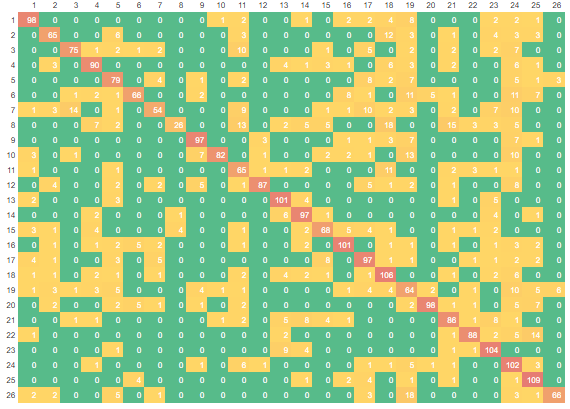
\includegraphics[width=\linewidth]{figs/confusion-matrix-letter-recognition-backpropagation-padrao.png}
  \caption{Confusion Matrix - Letter Recognition - Backpropagation padrão}
  \label{figura-confusion-matrix-letter-recognition-backpropagation-padrao}
\end{figure}

Os resultados para as 10 execuções do backpropagation padrão com as taxas de acertividade são apresentados na Tabela \ref{tabela-resultado-letter-recognition-backpropagation-padrao}. A média de acertividade foi de $0.7391$, com desvio padrão de $0.0062$.

\begin{table}[h!]
\centering
\caption{Resultados - Letter Recognition - Backpropagation padrão}
\label{tabela-resultado-letter-recognition-backpropagation-padrao}
\begin{tabular}{ll}
\toprule
                       & \textbf{Acertividade}       \\ \midrule
Execução 1             & 0.7363          \\
Execução 2             & 0.7370          \\
Execução 3             & 0.7380          \\
Execução 4             & 0.7527           \\
Execução 5             & 0.7360          \\
Execução 6             & 0.7353           \\
Execução 7             & 0.7367           \\
Execução 8             & 0.7477          \\
Execução 9             & 0.7380           \\
Execução 10            & 0.7330           \\ \bottomrule
\textbf{Média}         & \textbf{0.7391} \\
\textbf{Desvio Padrão} & \textbf{0.0062}
\end{tabular}
\end{table}

%O erro iterativo é apresentado na Figura \ref{figura-erro-iterativo-letter-recognition-backpropagation-padrao}.
%
%\begin{figure}
%  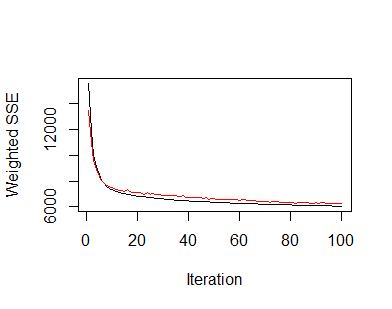
\includegraphics[width=\linewidth]{figs/erro-iterativo-letter-recognition-backpropagation-padrao.png}
%  \caption{Erro iterativo - Letter Recognition - Backpropagation padrão}
%  \label{figura-erro-iterativo-letter-recognition-backpropagation-padrao}
%\end{figure}

\subsubsection{SCG}

O backpropagation com função de aprendizado SCG foi executado para a base de dados Letter Recognition com os seguintes parâmetros:

\begin{itemize}
	\item \texttt{size}: 10
	\item \texttt{learnFuncParams}: (0, 0, 0, 0)
	\item \texttt{maxit}: 100
\end{itemize}

A confusion matrix de uma execução é apresentada na Figura \ref{figura-confusion-matrix-letter-recognition-backpropagation-scg}.

\begin{figure}[h!]
  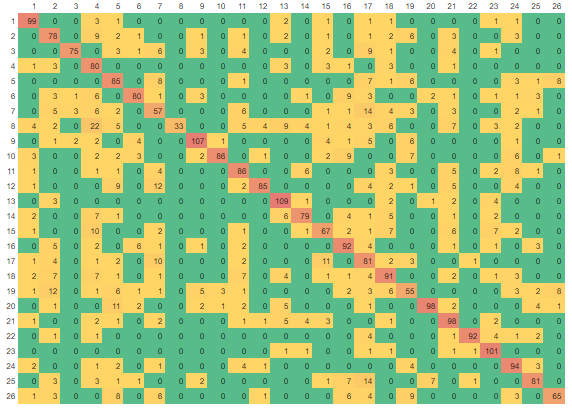
\includegraphics[width=\linewidth]{figs/confusion-matrix-letter-recognition-backpropagation-scg.png}
  \caption{Confusion Matrix - Letter Recognition - Backpropagation SCG}
  \label{figura-confusion-matrix-letter-recognition-backpropagation-scg}
\end{figure}

Os resultados para as 10 execuções do backpropagation SCG com as taxas de acertividade são apresentados na Tabela \ref{tabela-resultado-letter-recognition-scg}. A média de acertividade foi de $0.7262$, com desvio padrão de $0.0112$.

\begin{table}[h!]
\centering
\caption{Resultados - Letter Recognition - Backpropagation SCG}
\label{tabela-resultado-letter-recognition-scg}
\begin{tabular}{ll}
\toprule
                       & \textbf{Acertividade}       \\ \midrule
Execução 1             & 0.7430          \\
Execução 2             & 0.7280          \\
Execução 3             & 0.7187           \\
Execução 4             & 0.7117          \\
Execução 5             & 0.7203           \\
Execução 6             & 0.7327          \\
Execução 7             & 0.7163           \\
Execução 8             & 0.7257           \\
Execução 9             & 0.7207          \\
Execução 10            & 0.7453          \\ \bottomrule
\textbf{Média}         & \textbf{0.7262} \\
\textbf{Desvio Padrão} & \textbf{0.0112}
\end{tabular}
\end{table}

%O erro iterativo é apresentado na Figura \ref{figura-erro-iterativo-letter-recognition-backpropagation-scg}.
%
%\begin{figure}
%  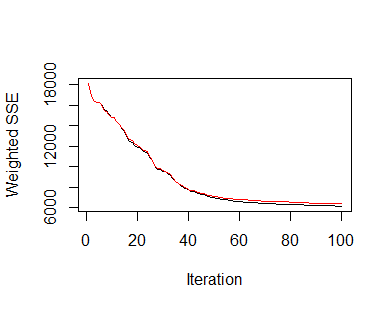
\includegraphics[width=\linewidth]{figs/erro-iterativo-letter-recognition-backpropagation-scg.png}
%  \caption{Erro iterativo - Letter Recognition - Backpropagation SCG}
%  \label{figura-erro-iterativo-letter-recognition-backpropagation-scg}
%\end{figure}

\subsection{Wine}

\subsubsection{Backpropagation padrão}

O backpropagation padrão foi executado para a base de dados Wine com os seguintes parâmetros:

\begin{itemize}
	\item \texttt{size}: 5
	\item \texttt{learnFuncParams}: 0.1
	\item \texttt{maxit}: 50
\end{itemize}

A confusion matrix de uma execução é apresentada na Figura \ref{figura-confusion-matrix-wine-backpropagation-padrao}.

\begin{figure}[h!]
  \centering
  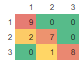
\includegraphics[width=0.3\linewidth]{figs/confusion-matrix-wine-backpropagation-padrao.png}
  \caption{Confusion Matrix - Wine - Backpropagation padrão}
  \label{figura-confusion-matrix-wine-backpropagation-padrao}
\end{figure}

Os resultados para as 10 execuções do backpropagation padrão com as taxas de acertividade são apresentados na Tabela \ref{tabela-resultado-wine-backpropagation-padrao}. A média de acertividade foi de $0.9630$, com desvio padrão de $0.0349$.

\begin{table}[h!]
\centering
\caption{Resultados - Wine - Backpropagation padrão}
\label{tabela-resultado-wine-backpropagation-padrao}
\begin{tabular}{ll}
\toprule
                       & \textbf{Acertividade}       \\ \midrule
Execução 1             & 1.0000          \\
Execução 2             & 0.9630          \\
Execução 3             & 0.9630          \\
Execução 4             & 0.9630           \\
Execução 5             & 0.9630          \\
Execução 6             & 1.0000           \\
Execução 7             & 0.9259           \\
Execução 8             & 0.9630          \\
Execução 9             & 0.8889           \\
Execução 10            & 1.0000           \\ \bottomrule
\textbf{Média}         & \textbf{0.9630} \\
\textbf{Desvio Padrão} & \textbf{0.0349}
\end{tabular}
\end{table}

%O erro iterativo é apresentado na Figura \ref{figura-erro-iterativo-wine-backpropagation-padrao}.
%
%\begin{figure}
%  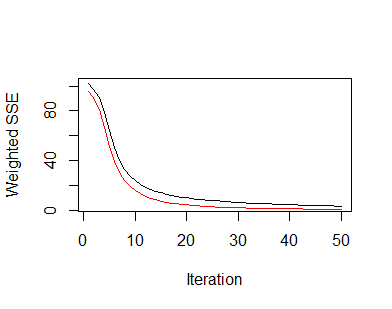
\includegraphics[width=\linewidth]{figs/erro-iterativo-wine-backpropagation-padrao.png}
%  \caption{Erro iterativo - Wine - Backpropagation padrão}
%  \label{figura-erro-iterativo-wine-backpropagation-padrao}
%\end{figure}

\subsubsection{SCG}

O backpropagation com função de aprendizado SCG foi executado para a base de dados Wine com os seguintes parâmetros:

\begin{itemize}
	\item \texttt{size}: 5
	\item \texttt{learnFuncParams}: (0, 0, 0, 0)
	\item \texttt{maxit}: 50
\end{itemize}

A confusion matrix de uma execução é apresentada na Figura \ref{figura-confusion-matrix-wine-backpropagation-scg}.

\begin{figure}[h!]
  \centering
  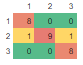
\includegraphics[width=0.3\linewidth]{figs/confusion-matrix-wine-backpropagation-scg.png}
  \caption{Confusion Matrix - Wine - Backpropagation SCG}
  \label{figura-confusion-matrix-wine-backpropagation-scg}
\end{figure}

Os resultados para as 10 execuções do backpropagation SCG com as taxas de acertividade são apresentados na Tabela \ref{tabela-resultado-wine-scg}. A média de acertividade foi de $0.9593$, com desvio padrão de $0.0273$.

\begin{table}[h!]
\centering
\caption{Resultados - Wine - Backpropagation SCG}
\label{tabela-resultado-wine-scg}
\begin{tabular}{ll}
\toprule
                       & \textbf{Acertividade}       \\ \midrule
Execução 1             & 1.0000          \\
Execução 2             & 0.9630          \\
Execução 3             & 0.9630           \\
Execução 4             & 0.9630          \\
Execução 5             & 0.9259           \\
Execução 6             & 0.9630          \\
Execução 7             & 0.9259           \\
Execução 8             & 0.9630           \\
Execução 9             & 0.9259          \\
Execução 10            & 1.0000          \\ \bottomrule
\textbf{Média}         & \textbf{0.9593} \\
\textbf{Desvio Padrão} & \textbf{0.0273}
\end{tabular}
\end{table}

%O erro iterativo é apresentado na Figura \ref{figura-erro-iterativo-wine-backpropagation-scg}.
%
%\begin{figure}
%  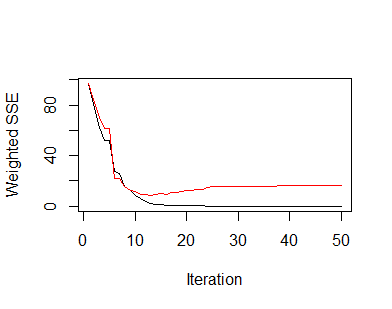
\includegraphics[width=\linewidth]{figs/erro-iterativo-wine-backpropagation-scg.png}
%  \caption{Erro iterativo - Wine - Backpropagation SCG}
%  \label{figura-erro-iterativo-wine-backpropagation-scg}
%\end{figure}

\subsection{Tic Tac Toe}

\subsubsection{Backpropagation padrão}

O backpropagation padrão foi executado para a base de dados Tic Tac Toe com os seguintes parâmetros:

\begin{itemize}
	\item \texttt{size}: 5
	\item \texttt{learnFuncParams}: 0.1
	\item \texttt{maxit}: 50
\end{itemize}

A confusion matrix de uma execução é apresentada na Figura \ref{figura-confusion-matrix-tic-tac-toe-backpropagation-padrao}.

\begin{figure}[h!]
  \centering
  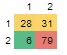
\includegraphics[width=0.3\linewidth]{figs/confusion-matrix-tic-tac-toe-backpropagation-padrao.png}
  \caption{Confusion Matrix - Tic Tac Toe - Backpropagation Padrão}
  \label{figura-confusion-matrix-tic-tac-toe-backpropagation-padrao}
\end{figure}

Os resultados para as 10 execuções do backpropagation padrão com as taxas de acertividade são apresentados na Tabela \ref{tabela-resultado-tic-tac-toe-backpropagation-padrao}. A média de acertividade foi de $0.7833$, com desvio padrão de $0.0401$.

\begin{table}[h!]
\centering
\caption{Resultados - Tic Tac Toe - Backpropagation padrão}
\label{tabela-resultado-tic-tac-toe-backpropagation-padrao}
\begin{tabular}{ll}
\toprule
                       & \textbf{Acertividade}       \\ \midrule
Execução 1             & 0.7500          \\
Execução 2             & 0.7986          \\
Execução 3             & 0.7500          \\
Execução 4             & 0.7778           \\
Execução 5             & 0.7500          \\
Execução 6             & 0.7500           \\
Execução 7             & 0.8194           \\
Execução 8             & 0.8403          \\
Execução 9             & 0.7500           \\
Execução 10            & 0.8472           \\
\textbf{Média}         & \textbf{0.7833} \\ \bottomrule
\textbf{Desvio Padrão} & \textbf{0.0401}
\end{tabular}
\end{table}

%O erro iterativo é apresentado na Figura \ref{figura-erro-iterativo-tic-tac-toe-backpropagation-padrao}.
%
%\begin{figure}
%  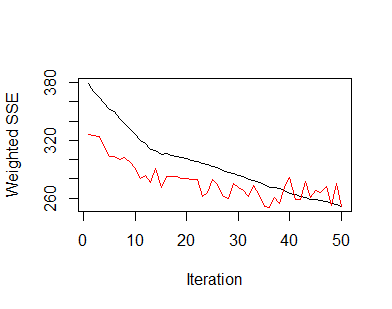
\includegraphics[width=\linewidth]{figs/erro-iterativo-tic-tac-toe-backpropagation-padrao.png}
%  \caption{Erro iterativo - Tic Tac Toe - Backpropagation Padrão}
%  \label{figura-erro-iterativo-tic-tac-toe-backpropagation-padrao}
%\end{figure}

\subsubsection{SCG}

O backpropagation com função de aprendizado SCG foi executado para a base de dados Tic Tac Toe com os seguintes parâmetros:

\begin{itemize}
	\item \texttt{size}: 5
	\item \texttt{learnFuncParams}: (0, 0, 0, 0)
	\item \texttt{maxit}: 50
\end{itemize}

A confusion matrix de uma execução é apresentada na Figura \ref{figura-confusion-matrix-tic-tac-toe-backpropagation-scg}.

\begin{figure}[h!]
  \centering
  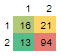
\includegraphics[width=0.3\linewidth]{figs/confusion-matrix-tic-tac-toe-backpropagation-scg.png}
  \caption{Confusion Matrix - Tic Tac Toe - Backpropagation SCG}
  \label{figura-confusion-matrix-tic-tac-toe-backpropagation-scg}
\end{figure}

Os resultados para as 10 execuções do backpropagation SCG com as taxas de acertividade são apresentados na Tabela \ref{tabela-resultado-wine-scg}. A média de acertividade foi de $0.7868$, com desvio padrão de $0.0656$.

\begin{table}[h!]
\centering
\caption{Resultados - Wine - Backpropagation SCG}
\label{tabela-resultado-wine-scg}
\begin{tabular}{ll}
\toprule
                       & \textbf{Acertividade}       \\ \midrule
Execução 1             & 0.7986          \\
Execução 2             & 0.7014          \\
Execução 3             & 0.9097           \\
Execução 4             & 0.7431          \\
Execução 5             & 0.6875           \\
Execução 6             & 0.8264          \\
Execução 7             & 0.8264           \\
Execução 8             & 0.7639           \\
Execução 9             & 0.8056          \\
Execução 10            & 0.8056          \\ \bottomrule
\textbf{Média}         & \textbf{0.7868} \\
\textbf{Desvio Padrão} & \textbf{0.0656}
\end{tabular}
\end{table}

%O erro iterativo é apresentado na Figura \ref{figura-erro-iterativo-tic-tac-toe-backpropagation-scg}.
%
%\begin{figure}
%  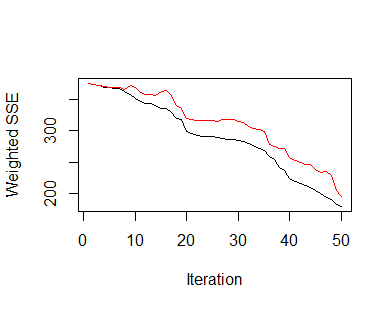
\includegraphics[width=\linewidth]{figs/erro-iterativo-tic-tac-toe-backpropagation-scg.png}
%  \caption{Erro iterativo - Tic Tac Toe - Backpropagation SCG}
%  \label{figura-erro-iterativo-tic-tac-toe-backpropagation-scg}
%\end{figure}

\subsection{Balance Scale}

\subsubsection{Backpropagation padrão}

O backpropagation padrão foi executado para a base de dados Balance Scale com os seguintes parâmetros:

\begin{itemize}
	\item \texttt{size}: 5
	\item \texttt{learnFuncParams}: 0.1
	\item \texttt{maxit}: 50
\end{itemize}

A confusion matrix de uma execução é apresentada na Figura \ref{figura-confusion-matrix-balance-scale-backpropagation-padrao}.

\begin{figure}[h!]
  \centering
  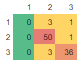
\includegraphics[width=0.3\linewidth]{figs/confusion-matrix-balance-scale-backpropagation-padrao.png}
  \caption{Confusion Matrix - Balance Scale - Backpropagation padrão}
  \label{figura-confusion-matrix-balance-scale-backpropagation-padrao}
\end{figure}

Os resultados para as 10 execuções do backpropagation padrão com as taxas de acertividade são apresentados na Tabela \ref{tabela-resultado-balance-scale-backpropagation-padrao}. A média de acertividade foi de $0.8713$, com desvio padrão de $0.0267$.

\begin{table}[h!]
\centering
\caption{Resultados - Balance Scale - Backpropagation padrão}
\label{tabela-resultado-balance-scale-backpropagation-padrao}
\begin{tabular}{ll}
\toprule
                       & \textbf{Acertividade}       \\ \midrule
Execução 1             & 0.8617          \\
Execução 2             & 0.8617          \\
Execução 3             & 0.8511          \\
Execução 4             & 0.9255           \\
Execução 5             & 0.8723          \\
Execução 6             & 0.8298           \\
Execução 7             & 0.8723           \\
Execução 8             & 0.9043          \\
Execução 9             & 0.8617           \\
Execução 10            & 0.8723           \\ \bottomrule
\textbf{Média}         & \textbf{0.8670} \\
\textbf{Desvio Padrão} & \textbf{0.0267}
\end{tabular}
\end{table}

%O erro iterativo é apresentado na Figura \ref{figura-erro-iterativo-balance-scale-backpropagation-padrao}.
%
%\begin{figure}
%  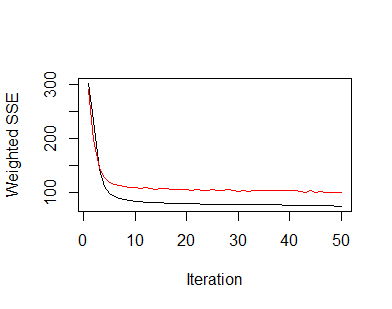
\includegraphics[width=\linewidth]{figs/erro-iterativo-balance-scale-backpropagation-padrao.png}
%  \caption{Erro iterativo - Balance Scale - Backpropagation Padrão}
%  \label{figura-erro-iterativo-balance-scale-backpropagation-padrao}
%\end{figure}

\subsubsection{SCG}

O backpropagation com função de aprendizado SCG foi executado para a base de dados Balance Scale com os seguintes parâmetros:

\begin{itemize}
	\item \texttt{size}: 5
	\item \texttt{learnFuncParams}: (0, 0, 0, 0)
	\item \texttt{maxit}: 50
\end{itemize}

A confusion matrix de uma execução é apresentada na Figura \ref{figura-confusion-matrix-balance-scale-backpropagation-scg}.

\begin{figure}[h!]
  \centering
  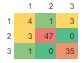
\includegraphics[width=0.3\linewidth]{figs/confusion-matrix-balance-scale-backpropagation-scg.png}
  \caption{Confusion Matrix - Balance Scale - Backpropagation SCG}
  \label{figura-confusion-matrix-balance-scale-backpropagation-scg}
\end{figure}

Os resultados para as 10 execuções do backpropagation SCG com as taxas de acertividade são apresentados na Tabela \ref{tabela-resultado-balance-scale-scg}. A média de acertividade foi de $0.9234$, com desvio padrão de $0.0425$.

\begin{table}[h!]
\centering
\caption{Resultados - Wine - Backpropagation SCG}
\label{tabela-resultado-balance-scale-scg}
\begin{tabular}{ll}
\toprule
                       & \textbf{Acertividade}       \\ \midrule
Execução 1             & 0.9149          \\
Execução 2             & 0.9043          \\
Execução 3             & 0.9574           \\
Execução 4             & 0.9255          \\
Execução 5             & 0.9574           \\
Execução 6             & 0.8191          \\
Execução 7             & 0.9574           \\
Execução 8             & 0.9468           \\
Execução 9             & 0.9468          \\
Execução 10            & 0.9043          \\ \bottomrule
\textbf{Média}         & \textbf{0.9234} \\
\textbf{Desvio Padrão} & \textbf{0.0425}
\end{tabular}
\end{table}

%O erro iterativo é apresentado na Figura \ref{figura-erro-iterativo-balance-scale-backpropagation-scg}.
%
%\begin{figure}
%  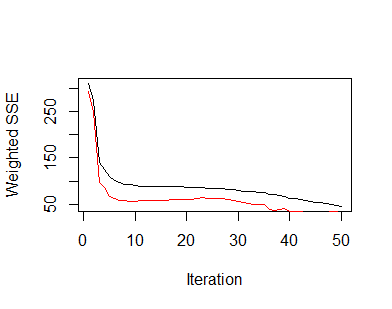
\includegraphics[width=\linewidth]{figs/erro-iterativo-balance-scale-backpropagation-scg.png}
%  \caption{Erro iterativo - Balance Scale - Backpropagation SCG}
%  \label{figura-erro-iterativo-balance-scale-backpropagation-scg}
%\end{figure}


\section{Conclusões}

A Tabela \ref{tabela-indices-acertividade} apresenta os índices de acertividade médios de todas as execuções. 

Nela é possível perceber que o Backpropagation Padrão teve melhores resultados em duas das bases de dados, enquanto o Backpropagation SCG teve melhor desempenho nas outras três. Na média, a função SCG tem um melhor desempenho em comparação com o Backpropagation Padrão. Nos experimentos realizado, há uma melhora de cerca de $1,13\%$.

\begin{table}[h!]
\centering
\caption{Índices de acertividade}
\label{tabela-indices-acertividade}
\begin{tabular}{@{}llll@{}}
\toprule
\textbf{Base de Dados} & \textbf{Padrão} & \textbf{SCG} & \textbf{Comparação} \\ \midrule
Iris                   & 0.9609                          & 0.9739 & 1.0135                       \\
Letter Recognition     & 0.7391                          & 0.7262 & 0.9825                      \\
Wine                   & 0.9630                          & 0.9593 & 0.9962                       \\
Tic Tac Toe            & 0.7833                          & 0.7868 & 1.0045                       \\
Balance Scale          & 0.8713                          & 0.9234 & 1.0598                       \\ \bottomrule
\textbf{Média}		   & \textbf{0.8635}							 & \textbf{0.8739} & \textbf{1.0113}
\end{tabular}
\end{table}

\section{Bibliografia}

\begin{thebibliography}{9}

\bibitem{bib-braga}
Braga, A. de P., "Redes neurais artificiais: teoria e aplica{\c{c}}{\~o}es" LTC Editora, 2007.

\bibitem{bib-moller}
Moller, Martin Fodslette. A scaled conjugate gradient algorithm for fast supervised learning.

\bibitem{bib-rsnns}
\url{https://github.com/cran/RSNNS/}

\bibitem{bib-iris}
\url{https://archive.ics.uci.edu/ml/datasets/Iris}

\bibitem{bib-letter-recognition}
\url{https://archive.ics.uci.edu/ml/datasets/Letter+Recognition}

\bibitem{bib-wine}
\url{https://archive.ics.uci.edu/ml/datasets/Wine}

\bibitem{bib-tic-tac-toe}
\url{https://archive.ics.uci.edu/ml/datasets/Tic-Tac-Toe+Endgame}

\bibitem{bib-balance-scale}
\url{https://archive.ics.uci.edu/ml/datasets/Balance+Scale}

\bibitem{bib-fisher}
Fisher,R.A. "The use of multiple measurements in taxonomic problems"
  Annual Eugenics, 7, Part II, 179-188 (1936); also in "Contributions
  to Mathematical Statistics" (John Wiley, NY, 1950).

\bibitem{bib-frey}
P. W. Frey and D. J. Slate (Machine Learning Vol 6 \#2 March 91):
	"Letter Recognition Using Holland-style Adaptive Classifiers".

\bibitem{bib-forina}
Forina, M. et al, PARVUS - An Extendible Package for Data
	Exploration, Classification and Correlation. Institute of Pharmaceutical
	and Food Analysis and Technologies, Via Brigata Salerno, 
	16147 Genoa, Italy.

\bibitem{bib-matheus}
Matheus,~C.~J., \& Rendell,~L.~A. (1989).  Constructive
	induction on decision trees.  In {\it Proceedings of the
	Eleventh International Joint Conference on Artificial Intelligence} 
	(pp. 645--650).  Detroit, MI: Morgan Kaufmann.

\end{thebibliography}

\end{document}